
\documentclass{beamer}
\usetheme{Madrid}
\usepackage[utf8]{inputenc}
\usepackage[spanish]{babel}
\usepackage{lmodern}
\usepackage{graphicx}
\usepackage{amsmath, amssymb}

\title{Análisis Predictivo y Gestión de Datos}
\subtitle{Sesión 7: Comparación de modelos e introducción a redes neuronales}
\author{Oscar Leonardo Rincón León}
\date{\today}

\begin{document}

\begin{frame}
  \titlepage
\end{frame}

\begin{frame}{Objetivo}
  Comparar modelos supervisados e introducir redes neuronales multicapa usando \texttt{MLPClassifier}.
\end{frame}

\begin{frame}{¿Por qué comparar modelos?}
  \begin{itemize}
    \item No todos los modelos funcionan igual para todos los datos.
    \item Comparar modelos permite detectar cuál generaliza mejor.
    \item Ayuda a justificar decisiones en análisis predictivo.
  \end{itemize}
\end{frame}

\begin{frame}{Estrategias de comparación}
  \begin{itemize}
    \item Usar la misma métrica de evaluación (ej. F1, AUC).
    \item Aplicar los modelos sobre los mismos datos.
    \item Usar validación cruzada para evitar depender de una sola partición.
  \end{itemize}
\end{frame}

\begin{frame}{Resumen conceptual de modelos}
  \textbf{¿Qué modelos comparamos?}
  \begin{itemize}
    \item \textbf{KNN}: clasificador basado en vecinos cercanos. Modelo perezoso, sensible a la escala.
    \item \textbf{Regresión logística}: modelo lineal para clasificación. Interpretable y eficiente.
    \item \textbf{Árbol de decisión}: modelo jerárquico. Captura no linealidades pero puede sobreajustar.
  \end{itemize}
\end{frame}

\begin{frame}{¿Qué es la validación cruzada?}
  \begin{itemize}
    \item Técnica para estimar el desempeño real de un modelo.
    \item Divide los datos en \texttt{k} particiones (folds).
    \item Se entrena sobre \texttt{k-1} partes y se evalúa sobre la restante, repitiendo el proceso.
    \item Reduce el sesgo de una única división de entrenamiento/prueba.
  \end{itemize}
\end{frame}

\begin{frame}{¿Qué es una red neuronal?}
  \begin{itemize}
    \item Modelo basado en capas de nodos (neuronas).
    \item Cada nodo aplica una función no lineal a una combinación de entradas.
    \item Tiene al menos una capa oculta entre entrada y salida.
    \item Aprende representaciones complejas de los datos.
  \end{itemize}
\end{frame}

\begin{frame}{Estructura de una red neuronal (MLP)}
  \begin{itemize}
    \item Capa de entrada: recibe las variables predictoras.
    \item Capas ocultas: aplican funciones no lineales.
    \item Capa de salida: da la predicción (por ejemplo, probabilidad de clase 1).
  \end{itemize}
  \begin{center}
    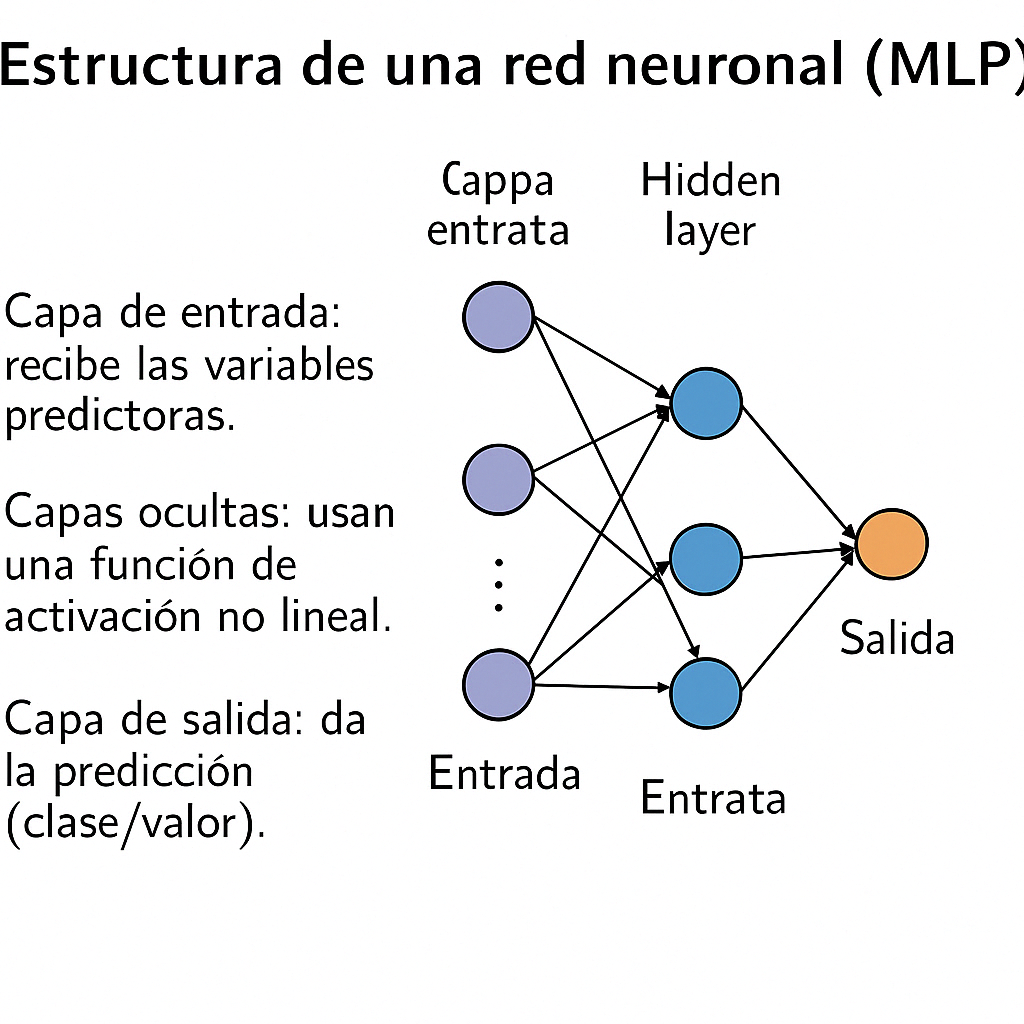
\includegraphics[width=0.55\textwidth]{mlp_architecture.png}
  \end{center}
\end{frame}

\begin{frame}{¿Qué es MLPClassifier?}
  \begin{itemize}
    \item Implementación de perceptrón multicapa en \texttt{scikit-learn}.
    \item Hiperparámetros:
    \begin{itemize}
      \item \texttt{hidden\_layer\_sizes}: número y tamaño de capas ocultas.
      \item \texttt{activation}: función de activación (ReLU, tanh, etc.).
      \item \texttt{solver}: algoritmo de optimización (ej. Adam).
    \end{itemize}
    \item Entrena con descenso del gradiente.
  \end{itemize}
\end{frame}

\begin{frame}{Ventajas y desventajas}
  \begin{block}{Ventajas}
    \begin{itemize}
      \item Captura relaciones no lineales complejas.
      \item Puede superar modelos tradicionales si se entrena bien.
    \end{itemize}
  \end{block}
  \begin{block}{Desventajas}
    \begin{itemize}
      \item Difícil de interpretar.
      \item Sensible a la selección de hiperparámetros.
    \end{itemize}
  \end{block}
\end{frame}

\begin{frame}{Resumen de la sesión}
  \begin{itemize}
    \item Se compararon modelos KNN, regresión logística y árboles.
    \item Se introdujo validación cruzada para evaluación más robusta.
    \item Se explicó la arquitectura de una red neuronal y el uso de \texttt{MLPClassifier}.
  \end{itemize}
\end{frame}

\end{document}
